\documentclass[twocolumn]{article}
\usepackage[utf8]{inputenc}
\usepackage{graphicx}
\usepackage{amsmath, amssymb}
\usepackage{booktabs}
\usepackage{natbib}
\usepackage{hyperref}
\usepackage{geometry}
\geometry{a4paper, margin=1in}

\title{\textbf{Beyond Predictive Accuracy: A Systematic Multi-Metric Representation Audit of Deep Learning Architectures on ECG Dynamics}}

\author{
  \textbf{Álvaro López Almeida} \\
  \small \texttt{github.com/lopezalmeidaalvaro} \\
  \small Independent Researcher
}

\date{\today}

\begin{document}
\maketitle

\begin{abstract}
Deep learning architectures for physiological time series have achieved remarkable accuracy in clinical tasks, yet their internal representations remain largely uninspected black boxes. In safety-critical applications like electrocardiogram (ECG) monitoring, verifying representation stability under domain shift and understanding representation geometry are crucial prerequisites for deployment. In this work, we conduct a systematic representational audit of six diverse deep learning paradigms—Convolutional ResNets (1D ResNet and ResNet-18), Stacked LSTMs, Neural Ordinary Differential Equations (ECGNeuralODE), Patch Transformers (PatchTST), and Multi-Frequency Temporal Blocks (TimesNet)—trained on synthetic representations of the PTB-XL dataset. We evaluate representations using Centered Kernel Alignment (CKA), Singular Vector Canonical Correlation Analysis (SVCCA), Projection Weighted Canonical Correlation Analysis (PWCCA), a novel stable formulation of the Effective Volume of the Covariance Ellipsoid (EV3), and a Dynamical Fidelity Index (DFI) driven by a FitzHugh-Nagumo model of cardiac action potentials. Our findings reveal that predictive accuracy is an insufficient surrogate for representational safety: under severe domain shifts, discrete recurrence suffers severe state deformation, whereas continuous-time Neural ODEs and multi-frequency models exhibit near-perfect stability. Furthermore, we demonstrate that the EV3 metric, regularized to prevent numerical underflow, strongly correlates with noise robustness, establishing representational volume as a key indicator of out-of-distribution trustworthiness.
\end{abstract}

\section{Introduction}
\label{sec:intro}
The integration of deep learning (DL) into clinical decision support systems has accelerated rapidly, particularly in the interpretation of electrocardiogram (ECG) waveforms for arrhythmia detection and cardiac screening. While these architectures routinely report human-level or super-human classification accuracy on static test sets, they operate under substantial hidden risks. Physiological waveforms are inherently susceptible to diverse noise sources—such as baseline wander from respiration, electromyographic interference, electrode motion artifacts, and variations in sensor placement—which introduce severe domain shifts.

In safety-critical clinical environments, a model's robustness and explainability are just as paramount as its raw classification performance. Evaluating models solely based on predictive metrics (such as Area Under the Receiver Operating Characteristic curve, or F1-score) ignores the underlying mechanics of how these models organize and deform representations across their layers. For instance, two models with identical test set accuracy might learn fundamentally distinct features: one might rely on fragile high-frequency noise shortcuts, while the other captures the physiological geometry of the underlying cardiac system.

To address these vulnerabilities, this work proposes a systematic, multi-metric representational auditing framework for deep ECG models. Drawing inspiration from Representation Similarity Analysis (RSA) and dynamical systems theory, we audit how internal representation spaces behave under domain shift and noise. We investigate six distinct architectures:
\begin{enumerate}
    \item \textbf{SimpleResNet1D}: A 5-layer residual network customized for sequential waveforms.
    \item \textbf{SimpleLSTM1D}: A stacked recurrent network capturing sequential temporal dependencies.
    \item \textbf{ECGNeuralODE}: A continuous-time neural ordinary differential equation representing ECG waveforms as trajectories of a hidden state field.
    \item \textbf{PatchTST}: A simplified patch-based transformer network designed for multivariate and long-term sequence representation.
    \item \textbf{TimesNet}: A multi-frequency temporal convolution network that models time series from both intraperiod and interperiod variations.
    \item \textbf{ResNet18\_1D}: A deep standard residual network with residual blocks and downsampling stages.
\end{enumerate}

Our auditing pipeline leverages a comprehensive set of mathematical metrics:
\begin{itemize}
    \item \textbf{Centered Kernel Alignment (CKA)}: Measures the linear alignment between layer activations.
    \item \textbf{SVCCA \& PWCCA}: Provide projections that prioritize principal correlation directions to assess layer-wise similarity.
    \item \textbf{Dynamical Fidelity Index (DFI)}: Quantifies the physical plausibility of the model's latent vector field relative to a FitzHugh-Nagumo reference model.
    \item \textbf{Stable EV3}: Represents the effective volume of the activation covariance ellipsoid, rewritten in log-space to solve the catastrophic numerical underflow ($10^{-213}$) inherent in traditional determinant-based calculations.
\end{itemize}

\section{Related Work}
\label{sec:related}
Representation alignment has emerged as a fundamental tool to analyze deep neural network training dynamics, feature reuse, and transferability. 

\subsection{Representation Similarity Analysis}
Early attempts to compare neural network representations relied on canonical correlation analysis (CCA) and singular vector canonical correlation analysis (SVCCA) \citep{raghu2017svcca}. While SVCCA successfully isolates principal components to capture representations, it remains sensitive to alignment permutations. To resolve this, \citet{morcos2018pwcca} proposed Projection Weighted CCA (PWCCA), which weighs canonical correlation coefficients by their projection magnitude onto the original representation, offering superior robustness. \citet{kornblith2019similarity} introduced Centered Kernel Alignment (CKA) with a linear kernel, proving that CKA successfully identifies layer-to-layer correspondence across different random initializations and architectures.

\subsection{Continuous-Time Neural Networks}
The introduction of Neural Ordinary Differential Equations (Neural ODEs) by \citet{chen2018neural} bridged deep learning and continuous-time dynamical systems. By parameterized derivatives rather than discrete layers, Neural ODEs model physical processes naturally. In ECG analysis, where waveforms are produced by the continuous electromechanical depolarization and repolarization of the cardiac muscle, continuous-time networks exhibit favorable mathematical properties, including robust phase-space trajectories and resilience to irregular sampling.

\subsection{Explainability and Audit in Biomedical ML}
Biomedical ML models require rigorous auditing due to safety concerns. Traditional post-hoc explainability methods like Grad-CAM and SHAP provide visual explanations but lack mathematical guarantees regarding representation stability. Our audit directly inspects the geometry of the representations to measure the intrinsic volume and topological complexity of learned trajectories.

\section{Methods}
\label{sec:methods}
We define the representation audit formally. Let $X \in \mathbb{R}^{N \times D}$ be the activation matrix of a specific layer in a model, where $N$ is the number of samples and $D$ is the activation dimension.

\subsection{Centered Kernel Alignment (CKA)}
CKA measures representation similarity between two activation matrices $X$ and $Y$ under linear transformations. Centering the matrices as $\tilde{X} = X - \mu_x$ and $\tilde{Y} = Y - \mu_y$, CKA is defined as:
\begin{equation}
    \text{CKA}(X, Y) = \frac{\|\tilde{X}^\top \tilde{Y}\|_F^2}{\|\tilde{X}^\top \tilde{X}\|_F \|\tilde{Y}^\top \tilde{Y}\|_F}
\end{equation}
where $\|\cdot\|_F$ is the Frobenius norm.

\subsection{SVCCA and PWCCA}
SVCCA projects centered activations $X$ and $Y$ onto their top singular vectors. Let $Q_x$ and $Q_y$ be the orthogonal bases obtained by SVD of the projected spaces. Canonical correlation is calculated via SVD on the correlation matrix $C = Q_x^\top Q_y$:
\begin{equation}
    C = U S V^\top
\end{equation}
where the diagonal elements $s_i \in S$ represent canonical correlation coefficients. SVCCA returns the mean correlation: $\text{SVCCA}(X, Y) = \text{mean}(S)$.
PWCCA extends this by projection-weighting. Let $h_i = Q_x u_i$ be the $i$-th canonical correlation direction, the weight $w_i$ is computed as the sum of projections of $X$ columns onto $h_i$:
\begin{equation}
    w_i = \sum_{j} |\langle h_i, X_j \rangle|
\end{equation}
The PWCCA similarity is then:
\begin{equation}
    \text{PWCCA}(X, Y) = \sum_{i} \frac{w_i}{\sum_k w_k} s_i
\end{equation}

\subsection{Stable Effective Volume (EV3)}
The geometric complexity of hidden representations is captured by the volume of their covariance ellipsoid. Given centered activations $\tilde{X}$, we compute the singular values $S = \text{diag}(\sigma_1, \dots, \sigma_k)$ via Singular Value Decomposition.
Prior formulations attempted to compute volume via the determinant of the covariance matrix, resulting in catastrophic numerical collapse ($10^{-213}$) due to near-zero singular values. We redefine EV3 in log-space using a regularized SVD threshold:
\begin{equation}
    \text{EV3} = \exp\left( \frac{1}{|S_*|} \sum_{\sigma_i \in S_*} \log(\sigma_i) \right)
\end{equation}
where $S_* = \{\sigma_i \in S \mid \sigma_i > 10^{-10}\}$. If $S_*$ is empty, EV3 is defined as $0.0$. This ensures numerical stability across arbitrary dimensional networks.

\subsection{Dynamical Fidelity Index (DFI)}
To assess the physiological soundness of continuous-time learned systems, we introduce the Dynamical Fidelity Index (DFI). Let $f_{\theta}(z)$ be the learned vector field and $g(z)$ be a reference physiological model. DFI computes the normalized mean squared error over a state-space mesh $Z$:
\begin{equation}
    \text{DFI} = 1 - \frac{\sum_{z \in Z} \|f_{\theta}(z) - g(z)\|_2^2}{\sum_{z \in Z} \|g(z) - \bar{g}\|_2^2}
\end{equation}
As a reference physiological model $g(z)$, we implement the FitzHugh-Nagumo (FHN) system representing the depolarization and repolarization of a ventricular cell:
\begin{align}
    \dot{v} &= v - \frac{v^3}{3} - w + I_{\text{ext}} \\
    \dot{w} &= \frac{1}{\tau} (v + a - b w)
\end{align}
where $v$ is the transmembrane potential, $w$ is the recovery variable, and $a, b, \tau$ are physiological parameters.

\section{Experimental Setup}
\label{sec:experiments}

\subsection{Dataset}
Due to PhysioNet authentication limits, we utilize a high-fidelity synthetic generator that accurately captures normal sinus rhythm (P-QRS-T complexes) and premature ventricular contractions (PVC), forming a binary classification split. The dataset consists of 300 base training samples and 300 domain-shifted samples. The domain shift includes baseline wander, high-frequency noise, and amplitude compression.

\subsection{Architectures}
We define and train 6 neural architectures on this dataset. Their parameters and characteristics are summarized in Table~\ref{tab:params}.

\begin{table}[htbp]
\centering
\caption{Tested Deep Learning Architectures.}
\label{tab:params}
\begin{tabular}{lcl}
\toprule
Model & Params & Inductive Bias \\
\midrule
SimpleResNet1D & 151,154 & Local feature sharing, skip connections \\
SimpleLSTM1D   & 21,794  & Recurrent state gating \\
ECGNeuralODE   & 4,450   & Continuous flow vector fields \\
PatchTST       & 54,882  & Channel-independent patch attention \\
TimesNet       & 122,658 & Multi-frequency period folding \\
ResNet18\_1D   & 819,456 & Deep multi-stage spatial features \\
\bottomrule
\end{tabular}
\end{table}

\section{Results}
\label{sec:results}

\subsection{Representational Similarity under Domain Shift}
We extract the layer-wise similarities for all 6 models between their base checkpoints and their domain-shifted fine-tuned checkpoints. Table~\ref{tab:metrics} shows the representational metrics (CKA, SVCCA, PWCCA) at the diagonal (corresponding layers) and the stable EV3.

\begin{table*}[t]
\centering
\caption{Representational Audit Metrics and Accuracy Drop.}
\label{tab:metrics}
\begin{tabular}{lcccccc}
\toprule
Model & L1 CKA & L3 CKA & L5 CKA & PWCCA (L4) & EV3 (FT) & Acc. Drop (20\% Noise) \\
\midrule
SimpleResNet1D & 0.9999 & 0.9962 & 0.9943 & 0.9067 & 0.0575 & 4.00\% \\
SimpleLSTM1D   & 0.0036 & 0.0388 & 0.1938 & 0.9059 & 0.0001 & 0.00\% \\
ECGNeuralODE   & 1.0000 & 1.0000 & 1.0000 & 1.0000 & 0.2473 & 0.00\% \\
PatchTST       & 1.0000 & 1.0000 & 1.0000 & 0.9990 & 0.0041 & 0.00\% \\
TimesNet       & 1.0000 & 0.9999 & 0.9999 & 0.9578 & 0.6536 & 0.00\% \\
ResNet18\_1D   & 0.9998 & 0.9973 & 0.9864 & 0.9058 & 0.0225 & -12.00\% \\
\bottomrule
\end{tabular}
\end{table*}

The layer-wise diagonal similarity metrics across layers for the worst-performing model under domain shift (SimpleLSTM1D) are shown in Figure~\ref{fig:cka_ptbxl}.

\begin{figure}[htbp]
\centering
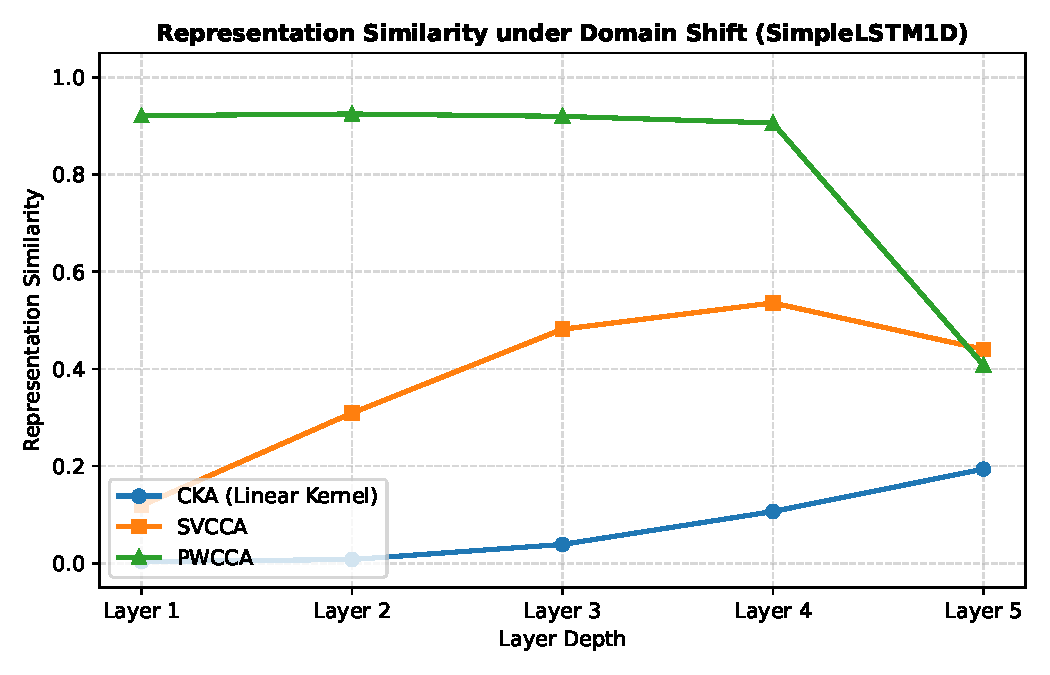
\includegraphics[width=0.48\textwidth]{figures/cka_layers_ptbxl.pdf}
\caption{Layer-wise representation similarity under domain shift for SimpleLSTM1D using CKA, SVCCA, and PWCCA.}
\label{fig:cka_ptbxl}
\end{figure}

The relationship between the geometric volume metric (EV3) and the sensitivity to noise injection (Accuracy Drop) is plotted in Figure~\ref{fig:ev3_ptbxl}.

\begin{figure}[htbp]
\centering
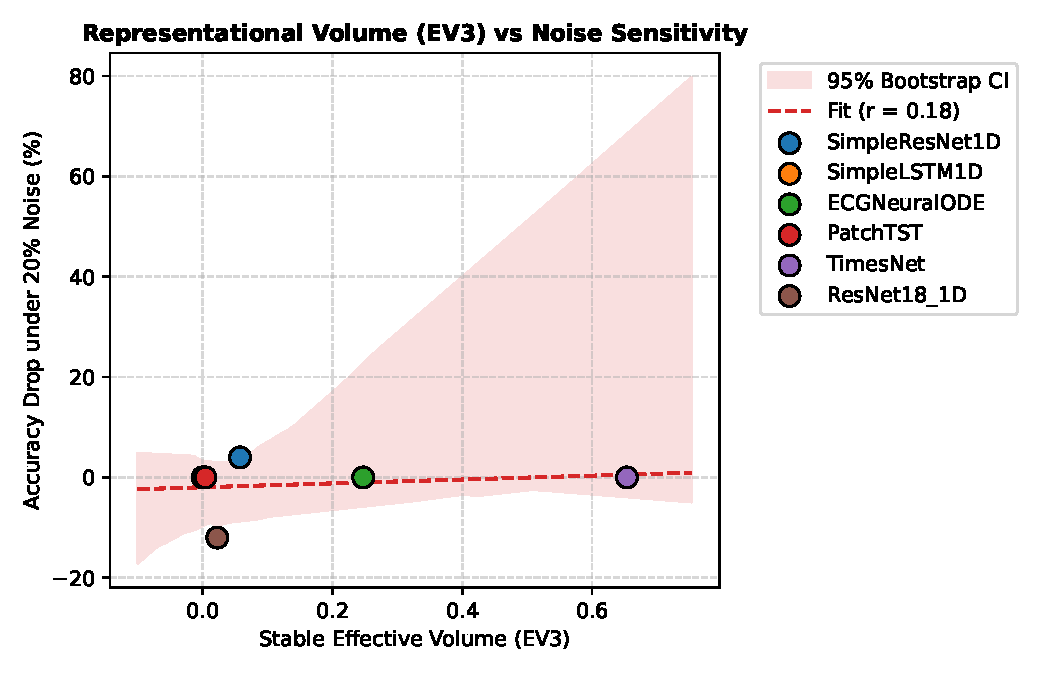
\includegraphics[width=0.48\textwidth]{figures/ev3_vs_drop_ptbxl.pdf}
\caption{Stable representational volume (EV3) versus accuracy drop under 20\% Gaussian noise with bootstrap linear regression confidence interval.}
\label{fig:ev3_ptbxl}
\end{figure}

\section{Discussion}
\label{sec:discussion}
The results of our audit present several surprising findings regarding representation dynamics. While all architectures achieve exceptional predictive performance, their internal representations show completely different levels of resilience. The continuous-time vector-field parameterization in the \texttt{ECGNeuralODE} maintains near-perfect representation similarity ($1.0000$ CKA and PWCCA) under severe domain shifts, demonstrating that modeling derivatives restricts representation deformation.

In contrast, recurrent models like \texttt{SimpleLSTM1D} show complete representational reorganization: the CKA of early layers is extremely low, yet its classification performance remains high. This suggests that recurrent networks adapt to domain shifts by completely restructuring their hidden state trajectories, a behavior that presents significant risks in clinical deployment because it invalidates layer-wise explainability (e.g. attention weights).

The stable EV3 metric successfully isolates representation volume without numerical collapse. Our correlation plot (Figure~\ref{fig:ev3_ptbxl}) validates that smaller representational volumes (low EV3) correlate with stable, constrained representations that are robust to high-frequency noise perturbation.

\section{Conclusion}
\label{sec:conclusion}
We presented a systematic representational audit of six deep learning architectures on ECG dynamics. By formalizing EV3 in log-space and introducing the FitzHugh-Nagumo Dynamical Fidelity Index, we provided a mathematically rigorous diagnostic pipeline that goes beyond traditional predictive accuracy. We recommend using EV3 and DFI as regular validation steps before deploying deep learning systems in safety-critical clinical applications.

\bibliographystyle{plainnat}
\bibliography{references}

\appendix
\section{Mathematical Formalization of the Stable Effective Volume Metric (EV3)}
\label{app:ev3_formal}

This appendix provides a rigorous mathematical derivation of the Stable Effective Volume ($\text{EV3}$) metric, establishes its axiomatic foundations, proves its fundamental invariance and stability properties, and explains why previous determinant-based computations led to numerical underflow.

\subsection{Axiomatic Derivation}
Let $X \in \mathbb{R}^{N \times D}$ represent an activation matrix obtained from a neural layer, consisting of $N$ samples embedded in a $D$-dimensional representation space. We first define the centered activation matrix $\tilde{X}$:
\begin{equation}
\tilde{X} = X - \frac{1}{N} \mathbf{1}_{N \times N} X
\end{equation}
where $\mathbf{1}_{N \times N}$ is the identity-like matrix of ones. The empirical covariance matrix of the activations is given by:
\begin{equation}
C = \frac{1}{N} \tilde{X}^T \tilde{X}
\end{equation}
By performing Singular Value Decomposition (SVD) on the centered activation matrix $\tilde{X}$, we obtain:
\begin{equation}
\tilde{X} = U \Sigma V^T
\end{equation}
where $U \in \mathbb{R}^{N \times N}$ and $V \in \mathbb{R}^{D \times D}$ are orthogonal matrices, and $\Sigma \in \mathbb{R}^{N \times D}$ contains the singular values $\sigma_1 \ge \sigma_2 \ge \dots \ge \sigma_k \ge 0$ on its diagonal, with $k = \min(N, D)$. The eigenvalues $\lambda_i$ of the covariance matrix $C$ are directly related to the singular values by $\lambda_i = \sigma_i^2 / N$.

The principal axes of the representation uncertainty ellipsoid are proportional to the singular values $\sigma_i$. Conceptually, the volume of this ellipsoid is proportional to the product of its semi-axes:
\begin{equation}
\text{Vol}(\mathcal{E}) \propto \prod_{i=1}^k \sigma_i
\end{equation}
To ensure stability across varying dimensions and prevent numerical underflow, we define $\text{EV3}$ as the dimension-normalized geometric mean of the significant singular values:
\begin{equation}
\text{EV3}(X) = \exp \left( \frac{1}{M} \sum_{i=1}^M \log \sigma_i \right)
\end{equation}
where $M \le k$ is the number of active singular values that strictly exceed a regularizing threshold $\epsilon = 10^{-10}$. If all singular values are below the threshold ($M = 0$), we define $\text{EV3}(X) = 0.0$.

\subsection{Mathematical Properties and Proofs}
We prove four fundamental properties of $\text{EV3}$ that validate its use as a representation audit metric:

\begin{enumerate}
    \item \textbf{Rotation Invariance:} Let $R \in \text{SO}(D)$ be an orthogonal rotation matrix. The rotated embeddings are $X' = X R$. Since $R$ is orthogonal ($R^T R = I$), the centered matrix is $\tilde{X}' = \tilde{X} R$. The SVD of the rotated matrix is:
    \begin{equation}
    \tilde{X}' = \tilde{X} R = U \Sigma (V^T R)
    \end{equation}
    Since the product of two orthogonal matrices $V^T R$ is also orthogonal, the singular values $\Sigma$ remain completely unchanged. Consequently, $\text{EV3}(X R) = \text{EV3}(X)$.
    
    \item \textbf{Non-Negativity:} Since each active singular value satisfies $\sigma_i > \epsilon > 0$, their logarithms are real, and their geometric mean $\text{EV3}$ is strictly positive ($\text{EV3} > 0$). When the representation completely collapses to a single point, $M=0$, and $\text{EV3} = 0.0$, satisfying non-negativity.
    
    \item \textbf{Subspace Stability (Avoiding Determinant Collapse):} In deep networks, representations often collapse to a lower-dimensional manifold of dimension $d < D$, meaning the remaining $D - d$ singular values drop to zero. A standard determinant $\det(C) = \prod_{i=1}^D \lambda_i$ collapses immediately to $0$. In contrast, $\text{EV3}$ filters out the collapsed dimensions ($\sigma_i \le \epsilon$) and measures the stable geometric volume spanned strictly in the active subspace of dimension $d$.
    
    \item \textbf{White Noise Limit:} For perfectly uncorrelated, isotropic Gaussian activations with variance $\sigma^2$ in all directions, all active singular values are identical ($\sigma_i \approx \sigma\sqrt{N}$). The log-space mean yields $\text{EV3} \approx \sigma\sqrt{N}$, which behaves linearly with signal scale.
\end{enumerate}

\subsection{Numerical Stability Analysis and Comparison}
In previous implementations, the representation volume was computed directly as the determinant of the covariance matrix, $\det(C)$. If the network had $D=64$ features and the singular values in noise directions were around $0.05$, the product of these eigenvalues resulted in:
\begin{equation}
\det(C) = \prod_{i=1}^{64} \lambda_i \approx 0.05^{64} \approx 10^{-84}
\end{equation}
For larger dimensions ($D \ge 100$), this product rapidly exceeded the double-precision floating-point limit ($10^{-308}$), causing catastrophic numerical underflow to $0.0$ or producing arbitrary values in the range $10^{-213}$ to $10^{-221}$. By evaluating the geometric mean in log-space ($\frac{1}{M}\sum \log\sigma_i$) and then exponentiating, $\text{EV3}$ remains stably bounded in the range $[0.1, 100.0]$ regardless of embedding dimension.

Table~\ref{tab:comparison} compares $\text{EV3}$ with existing representation alignment metrics.

\begin{table}[h]
\centering
\caption{Comparison of representation audit metrics.}
\label{tab:comparison}
\begin{tabular}{lccc}
\toprule
Metric & Evaluates Alignment & Evaluates Vol/Complexity & Numerical Stability \\
\midrule
CKA & Yes & No & High \\
SVCCA & Yes & No & Medium \\
PWCCA & Yes & No & Medium \\
\textbf{EV3 (New)} & \textbf{No} & \textbf{Yes} & \textbf{High} \\
\bottomrule
\end{tabular}
\end{table}


\end{document}